% %% %%%%%%%%%%%%%%%%%%%%%%%%%%%%%%%%%%%%%%%%%%%%%%%%%%%%%%%%%%
% practica.tex
%
% Author:  Mauricio Matamoros
% License: MIT
%
% %% %%%%%%%%%%%%%%%%%%%%%%%%%%%%%%%%%%%%%%%%%%%%%%%%%%%%%%%%%%

% TEX-ROOT=references.bib
% CHKTEX-FILE 1
% CHKTEX-FILE 13
\documentclass[letterpaper,10.5pt]{article}
\usepackage[utf8]{inputenc}
\usepackage[T1]{fontenc}
\usepackage[english,spanish,mexico,es-lcroman]{babel}
% Standard packages
\usepackage{float}
\usepackage{ifthen}
\usepackage{xspace}
\usepackage{amsmath}
\usepackage{xstring}
\usepackage{wrapfig}
\usepackage{booktabs}
\usepackage{csquotes}
\usepackage{fancyhdr}
\usepackage{fancyvrb}
\usepackage{geometry}
\usepackage{graphicx}
\usepackage{lastpage}
\usepackage{listings}
\usepackage{multicol}
\usepackage{multirow}
\usepackage{tabularx}
\usepackage{algorithm}
\usepackage{textgreek}
\usepackage[justification=centering]{subcaption}
\usepackage{algpseudocode}
\usepackage[all]{nowidow}
\usepackage[inline]{enumitem}
\usepackage[usenames,dvipsnames]{xcolor}
% Packages to be loaded later
\usepackage{tikz}
\usepackage{cancel}
\usepackage{tcolorbox}
% Include fullpage images with \includepdf
% \usepackage{pdfpages}
% Referencing
\usepackage{varioref}
\usepackage{hyperref}
\usepackage[noabbrev,nameinlink,spanish]{cleveref}
\usepackage[square, comma, numbers, sort&compress]{natbib}


\newcommand{\lpar}{(}\newcommand{\rpar}{)} %CHKTEX 9
\newcommand{\IIC}{I\textsuperscript{2}C\xspace}
\newcommand{\GND}{\textsc{Gnd}\xspace}
\newcommand{\VCC}{\textsc{Vcc}\xspace}
\newcommand{\VDD}{\textsc{Vdd}\xspace}
\newcommand{\textbi}[1]{\textbf{\textit{#1}}}
\newcommand{\degreesC}[1]{%
	#1\textsuperscript{o}C\xspace{}%
}
\newcommand{\degreesF}[1]{%
	#1\textsuperscript{o}F\xspace{}%
}

% \newcommand{\VCC}{V\textsubscript{CC}\xspace{}}
% \newcommand{\GND}{\textsc{Gnd}\xspace{}}
% CHKTEX-FILE 26
% CHKTEX-FILE 36

\tcbuselibrary{most}
% \tcbuselibrary{listings,breakable}
% \usetikzlibrary{shadings,shadows}
% \usetikzlibrary{decorations.pathmorphing}
% \usetikzlibrary{patterns}
% \usetikzlibrary{spy}
% \usetikzlibrary{arrows.meta}

\newtcolorbox{importantbox}[1]{%
	enhanced,
	colback=red!5!white,%
	colframe=red!75!black,%
	fonttitle=\bfseries,%
	center title,
	title={#1},%
	drop fuzzy shadow
}

\newtcolorbox{marker}[1][]{%
	enhanced,
	before skip=2mm,after skip=3mm,
	boxrule=0.4pt,left=5mm,right=2mm,top=1mm,bottom=1mm,
	colback=yellow!50,
	colframe=yellow!20!black,
	sharp corners,rounded corners=southeast,arc is angular,arc=3mm,
%	underlay={%
%		\path[fill=tcbcolback!80!black] ([yshift=3mm]interior.south east)--++(-0.4,-0.1)--++(0.1,-0.2);
%		\path[draw=tcbcolframe,shorten <=-0.05mm,shorten >=-0.05mm] ([yshift=3mm]interior.south east)--++(-0.4,-0.1)--++(0.1,-0.2);
%		\path[fill=yellow!50!black,draw=none] (interior.south west) rectangle node[white]{\Huge\bfseries !} ([xshift=4mm]interior.north west);
%	},
	drop fuzzy shadow,#1
}

%CHKTEX-FILE 1
%CHKTEX-FILE 7
%CHKTEX-FILE 9
% Default fixed font does not support bold face
\DeclareFixedFont{\ttb}{T1}{txtt}{bx}{n}{8} % for bold
\DeclareFixedFont{\ttm}{T1}{txtt}{m}{n}{8}  % for normal

% Custom colors
\usepackage{color}
\definecolor{keywordsColor}{rgb}{0,0,0.5}
\definecolor{customColor}{rgb}{0.6,0,0}
\definecolor{stringColor}{rgb}{0,0.5,0}

% Code highlighting python
\renewcommand{\ttdefault}{pcr}
\lstset{
	language=Python,                              % the language of the code (can be overrided per snippet)
	backgroundcolor=\color{white},                % choose the background color
	basicstyle=\footnotesize\ttfamily,            % the size of the fonts that are used for the code
	breakatwhitespace=false,                      % sets if automatic breaks should only happen at whitespace
	breaklines=true,                              % sets automatic line breaking
	captionpos=t,                                 % sets the caption-position to bottom
	commentstyle=\color{gray},                    % comment style
	deletekeywords={},                            % if you want to delete keywords from the given language
%	escapeinside={\%*}{*)},                       % if you want to add LaTeX within your code
	extendedchars=true,                           % lets you use non-ASCII characters; for 8-bits encodings only, does not work with UTF-8
	frame=tb,                                     % adds a frame around the code
	keepspaces=true,                              % keeps spaces in text, useful for keeping indentation of code (possibly needs columns=flexible)
	keywordstyle=\color{keywordsColor}\bfseries,  % keyword style
	numbers=left,                                 % where to put the line-numbers; possible values are (none, left, right)
	numbersep=5pt,                                % how far the line-numbers are from the code
	numberstyle=\tiny\color{gray},                % the style that is used for the line-numbers
	rulecolor=\color{black},                      % if not set, the frame-color may be changed on line-breaks within not-black text (e.g. comments (green here))
	showspaces=false,                             % show spaces everywhere adding particular underscores; it overrides 'showstringspaces'
	showstringspaces=false,                       % underline spaces within strings only
	showtabs=false,                               % show tabs within strings adding particular underscores
	stepnumber=1,                                 % the step between two line-numbers. If it's 1, each line will be numbered
	stringstyle=\color{stringColor},              % string literal style
	tabsize=2,                                    % sets default tabsize to 2 spaces
	title=\lstname,                               % show the filename of files included with \lstinputlisting; also try caption instead of title
	columns=fixed,                                % Using fixed column width (for e.g. nice alignment)
	otherkeywords={self},                         % if you want to add more keywords to the set
	emphstyle=\color{customColor}\bfseries,       % Custom highlighting style
	emph={__init__,__main__,True,False,None},     % Custom highlighting keywords
	xleftmargin=1cm,                              % Left margin
	xrightmargin=1cm,                             % Right margin
	% Unicode compatibility
	inputencoding=utf8,
	literate={%
	            {Á}{{\'a}}1 {É}{{\'E}}1 {Í}{{\'I}}1 {Ó}{{\'O}}1 {Ú}{{\'U}}1%
	            {á}{{\'a}}1 {é}{{\'e}}1 {í}{{\'i}}1 {ó}{{\'o}}1 {ú}{{\'u}}1%
	            {À}{{\`A}}1 {È}{{\'E}}1 {Ì}{{\`I}}1 {Ò}{{\`O}}1 {Ù}{{\`U}}1%
	            {à}{{\`a}}1 {è}{{\`e}}1 {ì}{{\`i}}1 {ò}{{\`o}}1 {ù}{{\`u}}1%
	            {Ä}{{\"A}}1 {Ë}{{\"E}}1 {Ï}{{\"I}}1 {Ö}{{\"O}}1 {Ü}{{\"U}}1%
	            {ä}{{\"a}}1 {ë}{{\"e}}1 {ï}{{\"i}}1 {ö}{{\"o}}1 {ü}{{\"u}}1%
	            {Â}{{\^A}}1 {Ê}{{\^E}}1 {Î}{{\^I}}1 {Ô}{{\^O}}1 {Û}{{\^U}}1%
	            {â}{{\^a}}1 {ê}{{\^e}}1 {î}{{\^i}}1 {ô}{{\^o}}1 {û}{{\^u}}1% CHKTEX 19
	            {Ã}{{\~a}}1 {Ẽ}{{\~E}}1 {Ĩ}{{\~I}}1 {Õ}{{\~O}}1 {Ũ}{{\~U}}1 {Ñ}{{\~N}}1%
	            {ã}{{\~a}}1 {ẽ}{{\~e}}1 {ĩ}{{\~i}}1 {õ}{{\~o}}1 {ũ}{{\~u}}1 {ñ}{{\~n}}1%
	            {œ}{{\oe}}1 {Œ}{{\OE}}1 {æ}{{\ae}}1 {Æ}{{\AE}}1 {ß}{{\ss}}1%
	            {ç}{{\c c}}1 {Ç}{{\c C}}1 {ø}{{\o}}1 {å}{{\r a}}1 {Å}{{\r A}}1%
	            {€}{{\EUR}}1 {£}{{\pounds}}1 {×}{{\(\times\)}}1% CHKTEX 21
	            {°}{{\textsuperscript{o}}}1%
	            {¹}{{\textsuperscript{1}}}1%
	            {²}{{\textsuperscript{2}}}1%
	            {³}{{\textsuperscript{3}}}1%
	            {⁴}{{\textsuperscript{4}}}1% CHKTEX 19
	            {⁵}{{\textsuperscript{5}}}1% CHKTEX 19
	            {⁶}{{\textsuperscript{6}}}1% CHKTEX 19
	            {⁷}{{\textsuperscript{7}}}1% CHKTEX 19
	            {⁸}{{\textsuperscript{8}}}1% CHKTEX 19
	            {⁹}{{\textsuperscript{9}}}1% CHKTEX 19
	            {⁰}{{\textsuperscript{0}}}1% CHKTEX 19
%	            {A}{{\textAlpha}}1
	            {α}{{\textalpha}}1%
%	            {B}{{\textBeta}}1
	            {β}{{\textbeta}}1%
	            {Γ}{{\textGamma}}1
	            {γ}{{\textgamma}}1%
	            {Δ}{{\textDelta}}1
	            {δ}{{\textdelta}}1% CHKTEX 19
%	            {E}{{\textEpsilon}}1
	            {ϵ}{{\textepsilon}}1%
%	            {Z}{{\textZeta}}1
	            {ζ}{{\textzeta}}1%
%	            {H}{{\textEta}}1
	            {η}{{\texteta}}1%
	            {Θ}{{\textTheta}}1
	            {θ}{{\texttheta}}1%
%	            {I}{{\textIota}}1
	            {ι}{{\textiota}}1%
%	            {K}{{\textKappa}}1
	            {κ}{{\textkappa}}1%
	            {Λ}{{\textLambda}}1
	            {λ}{{\textlambda}}1%
%	            {M}{{\textMu}}1
	            {μ}{{\textmu}}1%
%	            {N}{{\textNu}}1
	            {ν}{{\textnu}}1%
	            {Ξ}{{\textXi}}1
	            {ξ}{{\textxi}}1%
%	            {O}{{\textOmikron}}1
%	            {o}{{\textomikron}}1%
	            {Π}{{\textPi}}1
	            {π}{{\textpi}}1%
%	            {P}{{\textRho}}1
	            {ρ}{{\textrho}}1%
	            {Σ}{{\textSigma}}1
	            {σ}{{\textsigma}}1%
%	            {T}{{\textTau}}1
	            {τ}{{\texttau}}1%
	            {ϒ}{{\textUpsilon}}1
	            {υ}{{\textupsilon}}1%
	            {Φ}{{\textPhi}}1
	            {ϕ}{{\textphi}}1%
%	            {X}{{\textChi}}1
	            {χ}{{\textchi}}1%
	            {Ψ}{{\textPsi}}1
	            {ψ}{{\textpsi}}1%
	            {Ω}{{\textOmega}}1
	            {ω}{{\textomega}}1%
	            {ζ}{{\varsigma}}1%
%	            {}{{\straightphi}}1%
%	            {}{{\scripttheta}}1%
%	            {}{{\straighttheta}}1%
%	            {}{{\straightepsilon}}1%
	         },
}

\lstdefinestyle{c_with_comments}%
{
	language     = c,
	morecomment  = [l]{//},
	morecomment  = [s]{/*}{*/},
	breaklines,
}

\lstdefinestyle{c_without_comments}%
{
	style        = c_with_comments,
	% numbers      = none,
	% keepspaces   = false,
	morecomment  = [l][\nullfont]{//},
	morecomment  = [is]{//}{\^^M},
	morecomment  = [is]{/*}{*/},
}

\lstdefinelanguage{conf}
{
	basicstyle=\ttfamily\small,
	columns=fullflexible,
	morecomment=[s][\color{Orchid}\bfseries]{[}{]},
	morecomment=[l]{\#},
	morecomment=[l]{;},
	commentstyle=\color{gray}\ttfamily,
	% morekeywords={},
	% otherkeywords={=,:},
	% keywordstyle={\color{Green}\bfseries}
}

% \captionsetup[lstlisting]{font={small,tt}}
\captionsetup[lstlisting]{%
	font={small},
}



\DefineVerbatimEnvironment{Verbatim}{Verbatim}{%
	fontsize=\footnotesize,%
	frame=leftline,%
	framesep=2em,    % separation between frame and text
}

\RecustomVerbatimCommand{\VerbatimInput}{VerbatimInput}{%
	fontsize=\footnotesize,
%	frame=lines,            % top and bottom rule only
	frame=leftline,         % left rule only
	numbers=left,           % Line numbers on the left
	numbersep=0.25em,       % Gap between numbers and verbatim lines
	xleftmargin=4em,        % Indentation to add at the start of each line
	xrightmargin=4em,       % Right margin to add after each line
	framesep=0.5em,         % separation between frame and text
	rulecolor=\color{Gray}, % Color of the lines
	labelposition=topline,  %
	samepage=false,         % When true, prevents verbatim environment from
	                        % being broken between pages
%	commandchars=\|\(\),    % escape character and argument delimiters for
	                        % commands within the verbatim
%	commentchar=*           % comment character
}


\hypersetup{
	hidelinks,
	colorlinks=true,
	linkcolor=Blue,
	filecolor=OliveGreen,
	urlcolor=RoyalPurple,
	pdfauthor={Mauricio Matamoros},
%	pdftitle={Práctica 0X – Fundamentos de Sistemas Embebidos},
% 	pdfsubject={The Subject},
% 	pdfkeywords={Some Keywords},
% 	pdfproducer={Latex with hyperref, or other system},
% 	pdfcreator={pdflatex, or other tool}
}

\captionsetup{%
	font=small
}

\geometry{%
	margin=2cm,
	% top=3cm,
	bottom=3cm,
	% left=2cm,
	% right=2cm,
	% inner=2cm,
	% outer=2cm,
	% headheight=,
	% footsep=,
	% footskip=,
}

\pagestyle{fancy}
\renewcommand{\headrulewidth}{0.0pt}
\lhead{}
\chead{}
\rhead{}
\lfoot{}
\cfoot{}
\rfoot{Página~\thepage~de~\pageref{LastPage}}

\crefname{table}{tabla}{tablas}
\Crefname{table}{Tabla}{Tablas}
\crefname{section}{sección}{secciones}
\Crefname{section}{Sección}{Secciones}
\crefname{subsection}{subsección}{subsecciones}
\Crefname{subsection}{Subsección}{Subsecciones}
\crefname{listing}{código de ejemplo}{códigos de ejemplo}
\Crefname{listing}{Código de Ejemplo}{Códigos de Ejemplo}
\renewcommand*{\lstlistingname}{Código ejemplo}


\author{\footnotesize Autor: José Mauricio Matamoros de Maria y Campos}
\title{Práctica 8:\\Control de temperatura en lazo cerrado\\de una lámpara incandecente\\usando Arduino y la Raspberry Pi\\
{\large Fundamentos de Sistemas Embebidos}}
\date{}

% Document body
\begin{document}
\maketitle

\section{Objetivo}%
\label{sec:objective}
El alumno aprenderá a controlar la temperatura de un entorno cerrado calentado una carga resistiva de alta potencia opto-acoplada a un microcontrolador por medio de un detector de cruce por cero, un TRIAC, y un sensor de temperatura LM35.

% %% %%%%%%%%%%%%%%%%%%%%%%%%%%%%%%%%%%%%%%%%%%%%%%%%%%%%%%%%%%
% intro.tex
%
% Author:  Mauricio Matamoros
% License: MIT
%
% %% %%%%%%%%%%%%%%%%%%%%%%%%%%%%%%%%%%%%%%%%%%%%%%%%%%%%%%%%%%
%!TEX root = ../practica.tex
%!TEX root = ../references.bib

% CHKTEX-FILE 1
% CHKTEX-FILE 13
% CHKTEX-FILE 46

\section{Introducción}%
\label{seq:introduction}
La presente práctica resume los pasos a seguir para modular la temperatura de un entorno cerrado usando un sensor de temperatura LM35 y un foco incandescente o carga resistiva de alta potencia modulada mediante un detector de cruce por cero y un TRIAC.
En particular, se interesa en la implementación de un controlador proporcional e interfaz \IIC entre un Arduino y una Raspberry Pi.

% %% %%%%%%%%%%%%%%%%%%%%%%%%%%%%%%%%%%%%%%%%%%%%%%%%%%%%%%%%%%
% intro-lamps.tex
%
% Author:  Mauricio Matamoros
% License: MIT
%
% %% %%%%%%%%%%%%%%%%%%%%%%%%%%%%%%%%%%%%%%%%%%%%%%%%%%%%%%%%%%
%!TEX root = ../practica.tex
%!TEX root = ../references.bib

% CHKTEX-FILE 1
% CHKTEX-FILE 13
% CHKTEX-FILE 46

\subsection{Lámparas, eficiencia y calor}%
\label{intro-lamps}
En general, una lámpara cuenta con tres características fundamentales que definen su desempeño:
\begin{enumerate}[nosep,label=\roman*\rpar]
	\item \textbf{Brillo}: Medido en \emph{lúmenes}, el brillo determina la cantidad de iluminación que la lámpara provee; es decir, la cantidad de lúmenes es directamente proporcional a la iluminación que la lámpara proveerá.
	De hecho, el lúmen (abreviado $lm$) es la unidad del Sistema Internacional para medir el brillo, medida de la cantida de luz visible emitida por una fuente por unidad de tiempo; y que no debe ser confundido con la potencia total irradiada que contempla todas las frecuenciasen el espectro electromagnético, visibles o no.

	\item \textbf{Potencia}: Medida en \emph{watts}, se refiere a la potencia de consumo del dispositivo, aproximado por el producto del voltaje por la corriente.
	Debe diferenciarse de la potencia de trabajo que corresponde al trabajo realizado por el dispositivo, en este caso la cantidad de energía convertida en luz, y de la potencia total disipada que corresponde a diferencia entre la potencia suministrada y el trabajo realizado, es decir la energía perdida como calor y absorbida por los materiales.

	\item \textbf{Temperatura}: Medida en \emph{Kelvin}, se refiere al color de la luz que emite el dispositivo y está asociada a la temperatura en Kelvin del filamento en una lámpara incandecente y a la percepción subjetiva o sensación de calor que esta luz produce.
	Esto produce un efecto contradictorio entre los valores numéricos y su descripción.
	Contrario al sentido común, se le llama luz cálida a las lámparas que emiten luz en el rango de 2700--3000K y que emiten una mayor cantidad de fotones en la zona rojiza del espectro de luz visible,
	mientras que las lámparas de luz fría irradian en el rango de 5000--6500K que corresponde a la zona azulada del espectro de luz visible.
	Por último, están las lámparas de luz neutra que irradian en la zona amarillo-verdosa del espectro de luz visible en el rango de los 3500--4100K.
	Es importante hacer notar que, contrario al sentido común, de estas tres características y para los objetivos de esta práctica, la temperatura de una lámpara es el factor menos relevante a tomar en cuenta, puesto que es la que menos contribuye a la generación de calor.
\end{enumerate}

La eficiencia de una lámpara se determina como la cantidad de lúmenes que esta puede suministrar por Watt.
Una lámpara teórica perfecta tendría que ser capaz de convertir el 100\% de la energía proporcionada (electrones) en luz (fotones), valor que se encuentra determinado en $683\sfrac{lm}{w}$.
Este valor se utiliza para calcular la eficiencia real de cualquier lámpara del tipo que sea, como los ejemplos mostrados en la \Cref{tbl:lamp-efficiency}.
% Para este cálculo se toma en cuenta que la energía de un fotón se determina por la fórmula $E = hf$, donde $h=6.62\times10^{-34}\frac{m^{2}kg}{s}$, la constante de Plank, y $f$ es la frecuencia de oscilación del fotón, que está asociada a su longitud de onda $\lambda$ con la proporción $c=\lambda f$ donde $c=2.998\times 10^{8}\sfrac{m}{s}$.
% La longitud de onda está asociada al color (en una lámpara no interesan fotones fuera del espectro de luz visible que va de 770 a 380 nanómetros), así que una lámpara de máxima eficiencia liberaría fotones con la máxima energía visible posible, es decir, a una longitud de onda $\lambda = 380\times10^{-9}m$ lo que implica una frecuencia
% \(
% f
% 	= \frac{c}{\lambda}
% 	= \frac{2.998\times 10^{8}\frac{\cancel{m}}{s}}{770\times10^{-9}\cancel{m}}
% 	= 7.89\times10^{-4}s^{-1}
% \).



\begin{table}[t]
	\centering
	\caption[Eficiencia comparativa de lámparas]%
	{Eficiencia comparativa de lámparas\footnote{%
	Información obtenida de \url{https://www.lamps-on-line.com/watts-to-lumens}}}%
	\label{tbl:lamp-efficiency}
	\begin{tabularx}{0.85\linewidth}{X c c c c S S}
	\toprule
	\multicolumn{1}{c}{\multirow{2}{*}{\bfseries Foco}} &
	\multicolumn{4}{c}{\bfseries Consumo [W]} &
	\multicolumn{1}{c}{\multirow{2}{*}{\bfseries Eficiencia
	$\left[\frac{\text{lm}}{\text{W}}\right]$}} &
	\multicolumn{1}{c}{\multirow{2}{*}{\bfseries Eficiencia [\%]}}  \\
	              & 1500lm & 1100lm & 800lm & 450lm &        &      \\
	\midrule
	Incandescente &    100 &     75 &    60 &    40 &   15.0 &  2.1 \\
	Fluorescente  &     20 &     15 &    11 &     7 &   75.0 & 10.9 \\
	LED           &     13 &      9 &     8 &     5 &  125.0 & 18.3 \\
	\bottomrule
	\end{tabularx}
\end{table}

Con una eficiencia del 2.1\%, la lámpara incandescente se vuelve la opción más eficiente para generar calor (que no luz), ya que por cada 100W suministrados, aproximadamente 98W se convertirán en calor.
Además, otros tipos de lámparas funcionan por medio de una electrónica compleja basada en inductores o \emph{clamppers} que, además de ser no-lineales, son incompatibles con el método de modulación de potencia por detección de cruce por cero que se estudió en la pŕactica anterior.

Aparece entonces la pregunta de por qué no usar una resistencia convencional de alta potencia para estufa capaz de convertir el 99.9\% de la energía suministrada en calor.
Esto es debido a varias razones.
Primero, por costos, ya que una lámpara incandescente es mucho más barata que otro tipo de generadores de claor.
Segundo, porque es mucho más sencillo aprender a controlar un dispositivo observable a simple vista en el cual el calor disipado será proporcional de forma lineal al brillo emitido.
El tercer factor es la seguridad, ya que las resistencias para estufa generan demasiado calor demasiado rápido y pueden ocasionar quemaduras y encender llamas en segundos.
Y, por último, porque las resistencias para estufa están diseñadas para operar con un termostato y una carga y no para calentar un entorno por convección, por lo que habría que acoplarle un disipador con ventilador.

Luego entonces, corresponde estimar el incremento de temperatura por segundo para un volúmen de $1dm^3$ (un litro).
Se sabe que un foco incandescente opera como un resistor lineal y que 1 Watt equivale a 1 Julio por segundo.
Por otro lado una caloría está definida como la cantidad de calor requerida para elevar la temperatura de un gramo de agua a 4°C un $\Delta T = 1^{o}C$ en condiciones de presión de una atmósfera estándar, aproximadamente unos $4.184J$.

Sin embargo, el incremento de temperatura por unidad de calor varía de material a material (por ejemplo, el metal se calienta más rápido que el agua).
Por ello, es necesario calcular el incremento de temperatura que que tendrá un determinado volúmen de aire por cada caloría de energía suministrada, lo cual se logra considerando el calor específico de cada material.
Se sabe que el calor específico del agua es:\footnotemark{}
\footnotetext{El lector notará que el valor proporcionado del calor específico del agua no conincide con el valor de una caloría $1cal=4.1813\frac{J}{gK} \neq 4.1813\frac{J}{gK} = c_{p_\text{agua}}$. Esto se debe a que el valor usado para calcular el incremento de temperatura de un volumen de aire considera una temperatura ambiente promedio de 25°C, es decir, agua a 25°C y no los 4°C usados para conocer el equivalente mecánico del calor calculado por Joule.}

\begin{equation}
\label{eqn:sh-water}
	c_{p_\text{agua}} = 1\frac{cal}{gK} = 4.1813\frac{J}{gK}
\end{equation}

\noindent mientras que el calor específico del aire es:

\begin{equation}
\label{eqn:sh-air}
	c_{p_\text{aire}} = 1.012\frac{J}{gK}
\end{equation}

\noindent por lo que igualando valores con la fórmula del calor específico $Q = mc_{p}\Delta T$ se tiene que:

\begin{equation*}
	m_{_\text{agua}}c_{p_\text{agua}}\Delta T_{_\text{agua}} = Q = m_{_\text{aire}}c_{p_\text{aire}}\Delta T_{_\text{aire}}
\end{equation*}

\noindent considerando un volúmen fijo de un litro ($1L=1\times10^{-3}m^{3}$) y la densidad $\rho=\frac{m}{V}$ de cada material:

\begin{align*}
	\cancel{V_{_\text{agua}}\bigg\rvert_{1L}}\rho_{_\text{agua}}c_{p_\text{agua}}\Delta T_{_\text{agua}}
	=&&Q&&=
	\cancel{V_{_\text{aire}}\bigg\rvert_{1L}}\rho_{_\text{aire}}c_{p_\text{aire}}\Delta T_{_\text{aire}}
	\\
	\rho_{_\text{agua}}c_{p_\text{agua}}\Delta T_{_\text{agua}}
	=&&Q&&=
	\rho_{_\text{aire}}c_{p_\text{aire}}\Delta T_{_\text{aire}}
\end{align*}

considerando $\rho_{_\text{agua}}=1000\frac{kg}{m^3}$ y como $\Delta^{o}C = \Delta K$, se tiene:
\begin{align*}
	\cancelto{\scriptscriptstyle 1000\frac{kg}{m^3}}{\rho}_{_\text{agua}}
	c_{p_\text{agua}}
	\Delta T_{_\text{agua}}
	&=
	\rho_{_\text{aire}}c_{p_\text{aire}}\Delta T_{_\text{aire}}
	\\
	\left(1000\frac{kg}{m^3}\right)c_{p_\text{agua}}
	&=
	\rho_{_\text{aire}}c_{p_\text{aire}}\Delta T_{_\text{aire}}
\end{align*}

\noindent despejando
\begin{equation}
\label{eqn:traise-equivalence}
	\frac{\Delta T_{_\text{aire}}}{\Delta T_{_\text{agua}}} =
	\frac{c_{p_\text{agua}}}{\rho_{_\text{aire}}c_{p_\text{aire}}}
	\times
	\left(1\times10^3\left[\frac{kg}{m^3}\right]\right)
\end{equation}

\noindent reemplazando valores donde la densidad promedio del aire de $1.225\frac{kg}{m^3}$ y los calores específicos del agua y del aire (véase \cref{eqn:sh-water,eqn:sh-air}) se obtiene:

\begin{align*}
	\frac{\Delta T_{_\text{aire}}}{\Delta T_{_\text{agua}}} &=
	\frac{4.1813\cancel{\frac{J}{gK}}}%
	{1.012\cancel{\frac{J}{gK}}\cdot 1.225\cancel{\frac{kg}{m^3}}}
	\times
	\left(1\times10^3\cancel{\left[\frac{kg}{m^3}\right]}\right)\\
	&=3.37\times10^3[1]
\end{align*}

\noindent o bien:

\begin{equation}
\label{eqn:traise-equivalence-final}
	\Delta T_{_\text{aire}} = 3.37\times10^3 \Delta T_{_\text{agua}}
\end{equation}

Ahora bien, si se administran 100 watts de potencia durante 1 segundo a 1 gramo de agua a temperatura ambiente, éste elevaría su temperatura en aproximadamente 24°C asumiendo un comportamiento lineal ($100Ws = 100J = 23.9cal$); pero si se tratase de un litro de agua ($\rho_{agua} = 1\times10^3\frac{kg}{m^3} = 1\frac{kg}{L}$), éste sólo elevaría su temperatura en 0.024°C por tratarse de mil veces más agua.
Sin embargo, interesa calentar aire y no agua.
Por fortuna, la \cref{eqn:traise-equivalence-final} nos permite conocer cuál sería el incremento de temperatura en el mismo volumen de aire.
Así, aplicar 100 watts de pontencia durante 1 segundo a 1 litro de aire a temperatura ambiente elevaría la temperatura del aire en:
\begin{align*}
	\Delta T_{_\text{aire}}
	&= 3.37\times10^3 \Delta T_{_\text{agua}}\bigg\rvert_{0.024^{o}C}\\
	&= (3.37\times10^3)(0.024)\left[^{o}C\right]\\
	&= (3370)(0.024)\left[^{o}C\right]\\
	&= 80.88^{o}C\\
\end{align*}

Siguiendo este mismo razonamiento, es posible generalizar una fórmula, la \Cref{eqn:pow-temp}, que permite estimar el incremento de temperatura $\Delta T$ de un volumen de aire (en litros) por watt de energía suministrado cada segundo.

\begin{align*}
	\Delta T_{_\text{aire}}
	&= 3.37\times10^3 \Delta T_{_\text{agua}}\bigg\rvert_{2.39\times10^{-4}\frac{^{o}C}{Ws}}\\
\end{align*}

\noindent es decir:

\begin{align}
	\Delta T
	&= w_{f}t\big(3.37\times10^3\big) \big(2.39\times10^{-4}\big)\left[\tfrac{^{o}C}{Ws}\right]\\
	&= w_{f}t\big(3.37\times10^3\big) \big(0.239\big)\left[\tfrac{^{o}C}{Ws}\right]\\
\label{eqn:pow-temp}
	&= 80.54\times10^{-2}\left[\tfrac{^{o}C}{Ws}\right]w_{f}t
\end{align}

\noindent donde $\Delta T$ es el incremento de temperatura en un volumen de un litro de aire, $w_f$ es la potencia de disipación del foco y $t$ es el tiempo durante el cual la potencia es suministrada.

Es importante mencionar que la fórmula de la \Cref{eqn:pow-temp} es únicamente una aproximación burda que se basa en asunciones bastante fuertes, como por ejemplo el considerar la densidad y el calor específico de los materiales como constante, lo cual es altamente inexacto en el caso de gases, los cuales tienden a expandirse y reducir su densidad al ser calentados.
Si se intentara implementar un control de lazo abierto sería necesario un modelo matemático mucho más exacto\footnotemark{} para que la temperatura real fuera lo más próxima posible al valor deseado; pero como se implementará un controlador de lazo cerrado, esta aproximación lineal será suficiente.
\footnotetext{Un modelo matemático más preciso tendría que, por lo menos, modelar el volúmen de aire con la ecuación del gas ideal $PV=nRT$ junto con las contribuciones de energía derivadas del recambio de aire en el medio no sellado, lo que invariablemente llevaría a una ecuación integrodiferencial.}

% %% %%%%%%%%%%%%%%%%%%%%%%%%%%%%%%%%%%%%%%%%%%%%%%%%%%%%%%%%%%
% intro-control.tex
%
% Author:  Mauricio Matamoros
% License: MIT
%
% %% %%%%%%%%%%%%%%%%%%%%%%%%%%%%%%%%%%%%%%%%%%%%%%%%%%%%%%%%%%
%!TEX root = ../practica.tex
%!TEX root = ../references.bib

% CHKTEX-FILE 1
% CHKTEX-FILE 13
% CHKTEX-FILE 46

\subsection{Control}%
\label{intro-control}

Un sistema de control cerrado es aquel que utiliza un sensor para medir la salida del sistema, calcular el error respecto al valor deseado, y así suministrar la entrada necesaria para reducir el error lo más posible.
Así cuando se habla de control cerrado de manera implícita se habla de sistemas retroalimentados: aquellos en los que la salida actual depende tanto de la entrada como de la salida anterior tal como semuestra en la \Cref{fig:closed-loop}.

\begin{figure}[H]
	\centering
	
\includegraphics[width=0.8\textwidth,height=3cm,keepaspectratio]{img/closed-loop.png}
	\caption{Un sistema en lazo cerrado}%
	\label{fig:closed-loop}
\end{figure}

Para contorlar un sistema con un control de lazo cerrado (en adelante \emph{sistema de control}) se necesita de tres componentes fundamentales: un sensor que convierta la salida del sistema en una señal $B(s)$ que el controlador pueda interpretar, un amplificador operacional en modo resta que calcule el error $E(s)$ entre el valor deseado o entrada $R(s)$ y el valor sensado $B(s)$, y un dispositivo controlador $G_{c}(s)$ que transforme el error $E(s)$ en la entrada $V(s)$ que necesita el sistema controlado o \emph{planta} $G_p(s)$ para producir la salida deseada $Y(s)$, tal como se ejemplifica en la \Cref{fig:control-loop}.

\begin{figure}[H]
	\centering
	
\includegraphics[width=0.8\textwidth,height=3cm,keepaspectratio]{img/control-loop.png}
	\caption{Un sistema de control en lazo cerrado}%
	\label{fig:control-loop}
\end{figure}

Debido a que los modelos de este tipo de sistemas son aproximados con funciones diferenciales, es común se utilicen transformadas como la de Laplace o Fourier para simplificar el análisis y poder modelar el controlador de forma un poco más fácil, además de que interesa mucho más conocer la respuesta en frecuencia del sistema.

Matemáticamente:

\begin{align}
	Y(s) &= E(s)G(s)%
	\tag{a}\label{eqn:sysmodel-y}\\[5pt]
	G(s) &= G_{c}(s)G_{p}(s)%
	\tag{b}\label{eqn:sysmodel-g}\\[5pt]
	E(s) &= R(s)-B(s)%
	\tag{c}\label{eqn:sysmodel-e}\\[5pt]
	B(s) &= Y(s)H(s)%
	\tag{d}\label{eqn:sysmodel-b}
\end{align}

Sustituyendo las \cref{eqn:sysmodel-e,eqn:sysmodel-g} en la \cref{eqn:sysmodel-y}:

\begin{align}
	Y(s) &= \big(G_{c}(s)G_{p}(s)\big)\big(R(s)-B(s)\big)
	\notag{}\\[5pt]%
	&= G_{c}(s)G_{p}(s)R(s)-G_{c}(s)G_{p}(s)B(s)
	\tag{e}\label{eqn:sysmodel-y2}
\end{align}

reemplazando las \cref{eqn:sysmodel-b} en la \cref{eqn:sysmodel-y2}:

\begin{align}
	Y(s) &=
		G_{c}(s)G_{p}(s)R(s)
		-
		G_{c}(s)G_{p}(s)\Big[Y(s)H(s)\Big]
	\tag{f}\label{eqn:sysmodel-y3}
\end{align}

agrupando y reordenando:
\begin{align*}
	Y(s) &=
		G_{c}(s)G_{p}(s)R(s) -
		G_{c}(s)G_{p}(s)Y(s)H(s)\\[5pt]
	Y(s) + G_{c}(s)G_{p}(s)Y(s)H(s) &=
		G_{c}(s)G_{p}(s)R(s)\\[5pt]
	Y(s)\Big[1 + G_{c}(s)G_{p}(s)H(s)\Big] &=
		G_{c}(s)G_{p}(s)R(s)\\[5pt]
	Y(s) &= \frac%
		{G_{c}(s)G_{p}(s)R(s)}%
		{1 + G_{c}(s)G_{p}(s)H(s)}\\[5pt]
\end{align*}

Con lo que finalmente se obtiene la \emph{función de transferencia de lazo cerrado} $T(s)$ para un sistema retroalimentado con control cerrado:

\begin{equation}
	T(s) = \frac{Y(s)}{R(s)} =
	\frac{G_{c}(s)G_{p}(s)}{1 + G_{c}(s)G_{p}(s)H(s)}
	\label{eqn:transfer}
\end{equation}

Esta aproximación tiene un problema fundamental: la solución analítica de este tipo de ecuaciones suele ser computacionalmente muy costoso, lo que implica que se requerirán procesadores más potentes con un mayor consumo.
Para resolver este problema, el análisis se realiza no en el contínuo, sino que se discretiza al sistema y se modela un control en tiempo discreto (o digital) usando la transformada Z.
Con este tipo de modelado, la solución de integrales se convierte en suma de valores y las diferenciales en restas, lo que reduce enormemente el costo computacional de la solución del modelo del sistema, típicamente reduciéndolo a unos cuantos productos de matrices.


% %% %%%%%%%%%%%%%%%%%%%%%%%%%%%%%%%%%%%%%%%%%%%%%%%%%%%%%%%%%%
% intro-control.tex
%
% Author:  Mauricio Matamoros
% License: MIT
%
% %% %%%%%%%%%%%%%%%%%%%%%%%%%%%%%%%%%%%%%%%%%%%%%%%%%%%%%%%%%%
%!TEX root = ../practica.tex
%!TEX root = ../references.bib

% CHKTEX-FILE 1
% CHKTEX-FILE 13
% CHKTEX-FILE 46

\subsubsection{Control On/Off}%
\label{sec:control-onoff}

Un \emph{On/Off control} o control por encendido-apagado es la técnicas de control má simple que existe.
Su principio de funcionamiento se basa en definir regiones de operación fuera de las cuales la operación de la planta se detiene.
En su versión más simple, un controlador on-off hará funcionar a la planta a máxima potencia hasta que la salida registrada supere un valor umbral (\emph{threshold}), momento en el que se reducirá la potencia de la planta, normalmente cortando el suministro de enegía o \emph{apagándola}.
La planta permanecerá apagada hasta que la salida del sistema se reduzca por debajo del umbral de operación, momento en el que el controlador volverá a poner la planta en operación a máxima potencia.

Este tipo de controlador se observa comúnmente en sistemas que responden lentamente a cambios y que tienden a almacenar mucha energía, como por ejemplo los calentadores de agua estacionarios donde el quemador se enciende hasta que la temperatura del agua se eleva hasta cierto nivel (ej.~80°C) y no se volverá a encender hasta que la temperatura registrada descienda por debajo de un umbral de operación (ej.~60°C).
Además, el mecanismo de doble umbral del calentador evita que el quemador se esté encendiendo constantemente con cambios pequeños de temperatura.

Formalmente,

\begin{equation}
V(t) =
	\begin{cases}
	r(t) & \text{si}\; \left\lvert e(t)\right\rvert \geq k\\
	0    & \text{si}\; \left\lvert e(t)\right\rvert < k\\
	\end{cases}
\end{equation}

El inconveniente principal de este tipo de controlador es que genera transiciones abruptas que tienden a desgastar los materiales, especialmente cuando se opera a altas frecuencias.
Además, con este tipo de controlador no es posible modular la entrada del sistema dentro del rango de operación, dado que las transiciones sólo se producen en los umbrales, por lo que una operación suave es imposible.
Es por esto que este tipo de controladores es raramente usado en aplicaciones industriales.

% %% %%%%%%%%%%%%%%%%%%%%%%%%%%%%%%%%%%%%%%%%%%%%%%%%%%%%%%%%%%
% intro-control-p.tex
%
% Author:  Mauricio Matamoros
% License: MIT
%
% %% %%%%%%%%%%%%%%%%%%%%%%%%%%%%%%%%%%%%%%%%%%%%%%%%%%%%%%%%%%
%!TEX root = ../practica.tex
%!TEX root = ../references.bib

% CHKTEX-FILE 1
% CHKTEX-FILE 13
% CHKTEX-FILE 46

\subsubsection{Control proporcional}%
\label{sec:control-p}
Un control es proporcional cuando la salida $v(t)$ del controlador es proporcional al error $e(t)$:
\begin{equation*}
v(t ) = K_{P} e(t)
\end{equation*}

\noindent o en el dominio de la frecuencia:

\begin{equation*}
V(s) = K_{P} E(s)
\end{equation*}

\noindent por lo tanto

\begin{equation}
G_{c}(s) = \frac{V(s)}{E(s)} = K_{P}
\label{eqn:ctrl-p}
\end{equation}

Al otorgar una señal de entrada proporcional al error, éste tipo de control opera como un amplificador de error que, al corregirse, afecta negativamente la respuesta transitoria del sistema.
Es por esto que, a pesar de que un controlador P es fácil de implementar y ajustar, suele venir acompañado de otros elementos que compensen la amplificación del error y las variaciones transitorias.

Cuando se utiliza un control proporcional~\Citep{Hernandez2010}:
\begin{itemize}[noitemsep]
	\item El tiempo de elevación experimenta una pequeña reducción.
	\item El máximo pico de sobreimpulso se incrementa.
	\item El amortiguamiento se reduce.
	\item El tiempo de asentamiento cambia en pequeña proporción.
	\item El error de estado estable disminuye con incrementos de ganancia.
	\item El tipo de sistema permanece igual.
\end{itemize}


% %% %%%%%%%%%%%%%%%%%%%%%%%%%%%%%%%%%%%%%%%%%%%%%%%%%%%%%%%%%%
% intro-control-pi.tex
%
% Author:  Mauricio Matamoros
% License: MIT
%
% %% %%%%%%%%%%%%%%%%%%%%%%%%%%%%%%%%%%%%%%%%%%%%%%%%%%%%%%%%%%
%!TEX root = ../practica.tex
%!TEX root = ../references.bib

% CHKTEX-FILE 1
% CHKTEX-FILE 13
% CHKTEX-FILE 46

\subsubsection{Control integral}%
\label{sec:control-i}
Un control es integral cuando la salida $v(t)$ del controlador es proporcional a la integral del error $e(t)$:

\begin{equation*}
v(t) = K_{I} \int e(t) dt
\end{equation*}

\noindent o en el dominio de la frecuencia:

\begin{equation*}
V(s) = \frac{K_I}{s} E(s)
\end{equation*}

\noindent por lo tanto

\begin{equation}
G_{c}(s) = \frac{V(s)}{E(s)} = \frac{K_I}{s}
\label{eqn:ctrl-i}
\end{equation}

El objetivo de un control integral es el de reducir el error de estado estable, aunque esta corrección viene a costa de sobrecorregir el error, por lo que la respuesta del sistema tiende a oscilatoria o incluso a volverse inestable.
Es por esto que un controlador I suele venir acompañado de otros elementos que ayuden a estabilizar el sistema y a reducir las oscilaciones.

Cuando se combina con un controlador tipo proporcional para formar un control PI \Citep{Hernandez2010}:
\begin{itemize}[noitemsep]
	\item El amortiguamiento se reduce.
	\item El máximo pico de sobreimpulso se incrementa.
	\item Decrece el tiempo de elevación.
	\item Se mejoran los márgenes de ganancia y fase.
	\item El tipo de sistema se incrementa en una unidad.
	\item El error de estado estable mejora por el incremento del tipo de sistema.
\end{itemize}


% %% %%%%%%%%%%%%%%%%%%%%%%%%%%%%%%%%%%%%%%%%%%%%%%%%%%%%%%%%%%
% intro-control-pd.tex
%
% Author:  Mauricio Matamoros
% License: MIT
%
% %% %%%%%%%%%%%%%%%%%%%%%%%%%%%%%%%%%%%%%%%%%%%%%%%%%%%%%%%%%%
%!TEX root = ../practica.tex
%!TEX root = ../references.bib

% CHKTEX-FILE 1
% CHKTEX-FILE 13
% CHKTEX-FILE 46

\subsubsection{Control derivativo}%
\label{sec:control-d}
Un control es derivativo cuando la salida $v(t)$ del controlador es proporcional a la derivada del error $e(t)$:

\begin{equation*}
v(t) = K_{D}\;\frac{d\;e(t)}{dt}
\end{equation*}

\noindent o en el dominio de la frecuencia:

\begin{equation*}
V(s) = K_{D}\;s\;E(s)
\end{equation*}

\noindent por lo tanto

\begin{equation}
G_{c}(s) = \frac{V(s)}{E(s)} = K_{D}s
\label{eqn:ctrl-d}
\end{equation}

Debido a que la derivada del error respecto al tiempo es la velocidad del error, un control derivativo se anticipará a los errores antes de que estos se produzcan, amortiguando oscilaciones.
Sin embargo, un controlador D es insensible a errores de estado estable, por lo que suele acompañarse de otros elementos que sí corrijan el error de estado estable.

Cuando se combina con un controlador tipo proporcional para formar un control PD \Citep{Hernandez2010}:
\begin{itemize}[noitemsep]
	\item El amortiguamiento se incrementa.
	\item El máximo pico de sobreimpulso se reduce.
	\item El tiempo de elevación experimenta pequeños cambios.
	\item Se mejoran el margen de ganancia y el margen de fase.
	\item El error de estado estable presenta pequeños cambios.
	\item El tipo de sistema permanece igual.
\end{itemize}


% %% %%%%%%%%%%%%%%%%%%%%%%%%%%%%%%%%%%%%%%%%%%%%%%%%%%%%%%%%%%
% intro-control-pid.tex
%
% Author:  Mauricio Matamoros
% License: MIT
%
% %% %%%%%%%%%%%%%%%%%%%%%%%%%%%%%%%%%%%%%%%%%%%%%%%%%%%%%%%%%%
%!TEX root = ../practica.tex
%!TEX root = ../references.bib

% CHKTEX-FILE 1
% CHKTEX-FILE 13
% CHKTEX-FILE 46

\subsubsection{Control PID digital}%
\label{sec:control-pid}
Un control \emph{proporcional-integral-derivativo} o PID incorpora las mejores características de los controles PI y PD, motivo por el cual ha sido uno de las técnicas de control continuo más utilizados en la industria por más de siete décadas \citep{Hernandez2010,Odwyer2009,Ogata2003}.

Con base en las ecuaciones \Cref{eqn:ctrl-p,sec:control-i,eqn:ctrl-d} el controlador sería de la forma:

\begin{equation}
G_{c}(s) = \frac{V(s)}{E(s)} =
	K_{P} + \frac{K_I}{s} + K_{D}s
\end{equation}

Sin embargo, como se mencionó anteriormente en la \Cref{intro-control}, integrar señales en tiempo contínuo es computacionalmente muy costoso.
Además, la señal del sensor pasará por un convertidor analógico-digital que discretizará la señal, por lo que tiene más sentido implementar un controlador discreto.
Luego entonces, interesa conocer el valor (también discreto) que se proporcionará a la planta para obtener la señal deseada en el sensor.
En el contínuo esta sería:

\begin{equation*}
v(t) = K_{P}\,e(t) + {K_I}\int e(t)\,dt+ K_{D}\frac{d\,e(t)}{dt}
\label{eqn:v-pid}
\end{equation*}

Si se muestrea el error a una intervalos de tiempo constante con frecunecia lo suficientemente alta, es posible convertir la \cref{eqn:v-pid} en una ecuación en diferencias sobre la $k$-ésima muestra tomada:

\begin{equation*}
v[k] =
		K_{P}\,e[k] +
		K_{I}\sum^{k}_{j=0} e[j]+
		K_{D}\big(e[k] - e[k-1]\big)
\end{equation*}

\noindent donde

\begin{align*}
	&e[k]                     && \text{el error actual}\\
	&e[k-1]                   && \text{el error anterior}
\end{align*}

Además, si se considera $P_{I}[k] = K_{I}\sum^{k}_{j=0} e[j]$ entonces:

\begin{align*}
P_{I}[k]
	&= K_{I}\sum^{k}_{j=0} e[j]\\
	&= K_{I}\,e[k] + P_{i}[k-1]
\end{align*}

Así, aproximar un control digital para un sistema simple puede ser tan sencillo como almacenar en memoria los últimos valores sensados del error y el acumulado de la componente integral del PID, lo que reduce el cómputo a sólo unas cuantas operaciones aritméticas simples: sumas, restas y productos.
No obstante, es necesario recordar que ésto no funcionará con sistemas que tengan una dinámica compleja, particularmente los no-lineales.






% CHKTEX-FILE 1
% CHKTEX-FILE 13
% CHKTEX-FILE 46
%!TEX root = ../practica.tex
%!TEX root = ../references.bib

%% %%%%%%%%%%%%%%%%%%%%%%%%%%%%%%%%%%%%%%%%%%%%%%%%%%%%%%%%%%%%%%%%%%
%
% Material
%
%% %%%%%%%%%%%%%%%%%%%%%%%%%%%%%%%%%%%%%%%%%%%%%%%%%%%%%%%%%%%%%%%%%%
\section{Material}%
\label{sec:material}
Se asume que el alumno cuenta con un una Raspberry Pi con sistema operativo Raspbian e interprete de Python instalado. Se aconseja encarecidamente el uso de \textit{git} como programa de control de versiones.

Además, el alumno necesitará los alambrados de la
\href{https://github.com/kyordhel/FSEm/tree/master/practica06}{Práctica 6}
y la
\href{https://github.com/kyordhel/FSEm/tree/master/practica07}{Práctica 7}.

\subsection{Lista de componentes}%
\label{sec:material-component-list}

\begin{itemize}[noitemsep]
	\item 1 Arduino UNO o Arduino Mega
	\item 1 sensor de temperatura LM35 en encapsulado TO-220 o TO-92
	\item 1 TRIAC BT138 o BT139
	\item 4 diodos 1N4007 o puente rectificador equivalente
	\item 2 diodos 1N914
	\item 1 optoacoplador MOC 3021
	\item 1 optoacoplador 4N25
	\item 1 foco incandescente (NO AHORRADOR NI LED)
	\item 1 resistencia de 15k$\Omega$
	\item 1 resistencia de 18k$\Omega$
	\item 1 resistencia de 12k$\Omega$\footnotemark
	\item 3 resistencia de 10k$\Omega$
	\item 2 resistencia de 4k7$\Omega$
	\item 1 resistencia de  1k$\Omega$
	\item 2 resistencia de 470$\Omega$
	\item 2 resistencia de 330$\Omega$
	\item 1 condensador de 0.1$\mu$F
	\item 1 pecera o caja de acrílico transparente o de cartulina blanca
	\item 1 protoboard o circuito impreso equivalente
	\item 1 fuente de alimentación regulada a 5V y al menos 2 amperios de salida
	\item Cables y conectores varios
\end{itemize}

\footnotetext{La resistencia de 12k$\Omega$ puede reemplazarse con resistencias de 13k$\Omega$ a 20k$\Omega$ dependiendo del voltaje de los diodos.} %chktex 42

% \cleardoublepage
% %% %%%%%%%%%%%%%%%%%%%%%%%%%%%%%%%%%%%%%%%%%%%%%%%%%%%%%%%%%%
% steps.tex
%
% Author:  Mauricio Matamoros
% License: MIT
%
% %% %%%%%%%%%%%%%%%%%%%%%%%%%%%%%%%%%%%%%%%%%%%%%%%%%%%%%%%%%%
%!TEX root = ../practica.tex
%!TEX root = ../references.bib

% CHKTEX-FILE 1
% CHKTEX-FILE 13
% CHKTEX-FILE 46

\section{Instrucciones}%
\label{sec:instructions}
\begin{enumerate}[noitemsep]
	\item Alambre el circuito mostrado en las \Cref{fig:circuit-dc,fig:circuit-ac}.
	\item Realice los programas de la \Cref{sec:step3}
 	\item Analice los programas de la \cref{sec:step3} y realice los experimentos propuestos en la \cref{sec:experiments}.
 	% y con los resultados obtenidos responda el cuestionario de la \cref{sec:questionnaire}.
\end{enumerate}

% %% %%%%%%%%%%%%%%%%%%%%%%%%%%%%%%%%%%%%%%%%%%%%%%%%%%%%%%%%%%
% step-1.tex
%
% Author:  Mauricio Matamoros
% License: MIT
%
% %% %%%%%%%%%%%%%%%%%%%%%%%%%%%%%%%%%%%%%%%%%%%%%%%%%%%%%%%%%%
%!TEX root = ../practica.tex
%!TEX root = ../references.bib

% CHKTEX-FILE 1
% CHKTEX-FILE 13
% CHKTEX-FILE 46

\subsection{Implementación un controlador On/Off}%
\label{sec:step-1}

Alambre cuidadosamente los circuitos de las prácticas \href{https://github.com/kyordhel/FSEm/tree/master/practica06}{6} y \href{https://github.com/kyordhel/FSEm/tree/master/practica07}{7} para crear un circuito AC-DC optoacoplado completo para control cerrado de temperatura usando un foco incandescente operado con un LM35 y un circuito de variación de fase mediante detección de cruce por cero.
El circuito completo alambrado debe verse como el de la \Cref{fig:circuit-full}.

\medskip

\begin{importantbox}{\large Importante}
	\begin{center}
		Asegúrese de verificar con un multímetro que el circuito de AC está debidamente aislado y que no se tienen valores mayores a 5V en el segmento de DC.
		De otro modo podría quemar su Arduino y su Raspberry Pi.
	\end{center}
\end{importantbox}

\medskip

\begin{figure}
	\centering
	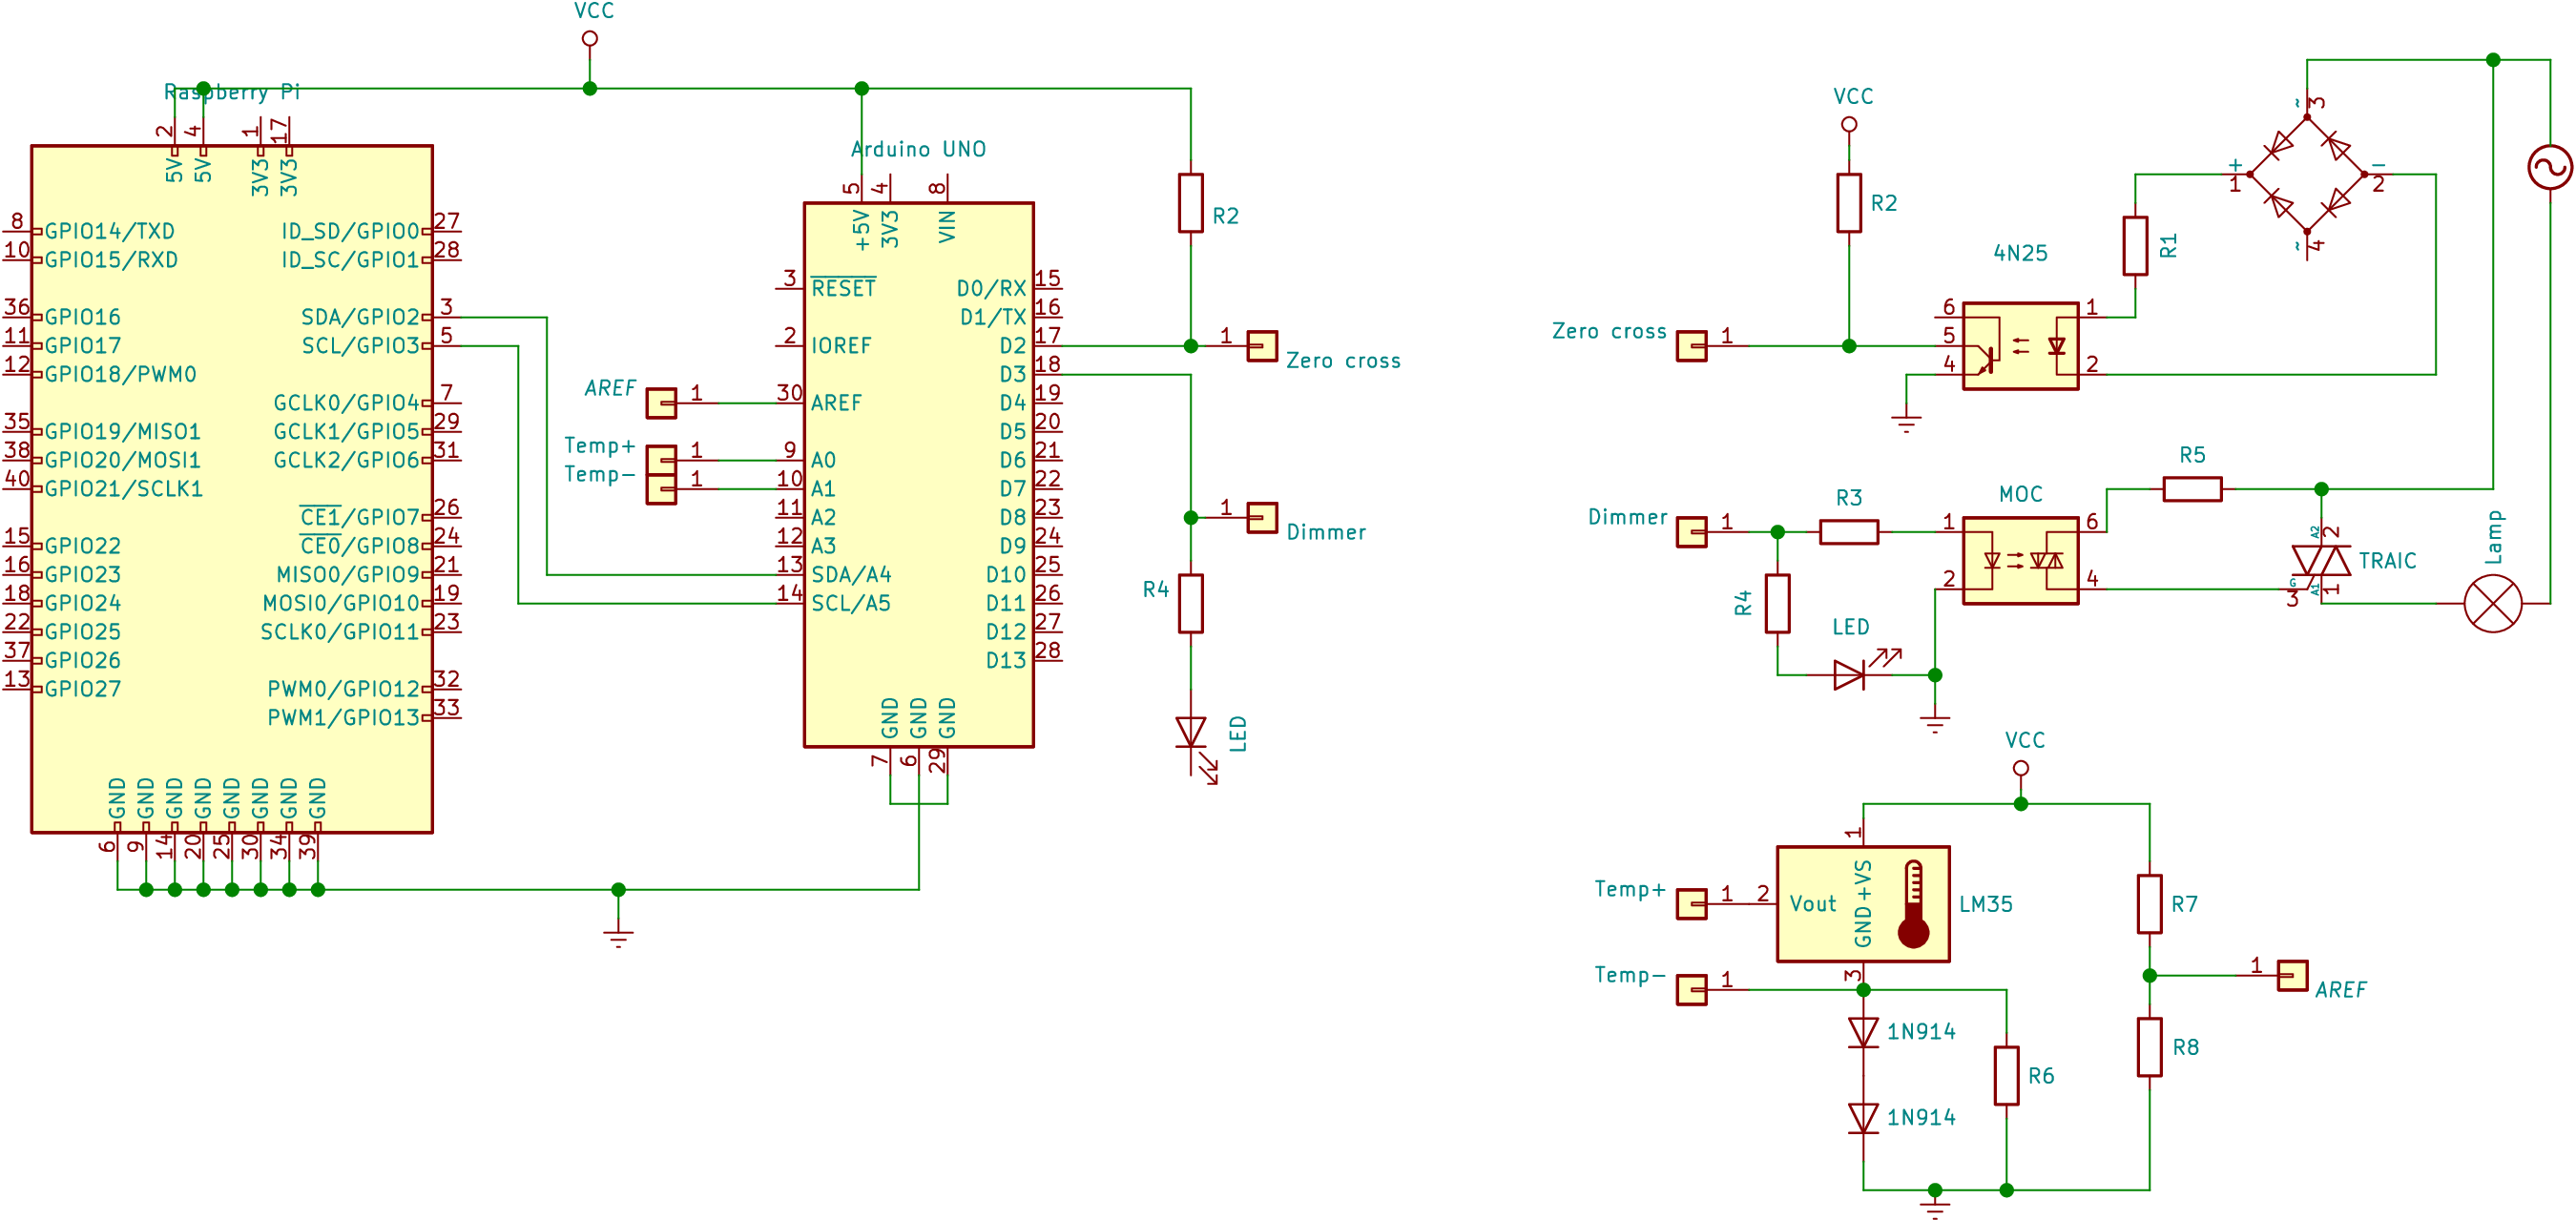
\includegraphics[width=0.85\linewidth,height=6cm,keepaspectratio]{img/circuit-full.png}
	\caption{Circuito AC-DC optoacoplado completo para control cerrado de temperatura.}%
	\label{fig:circuit-full}
\end{figure}

De acuerdo con el alambrado de la \Cref{fig:circuit-full}, el Arduino ha de realizar tres funciones:
\begin{enumerate*}[label=\roman*\rpar]
	\item digitalización del valor de temperatura analógico sensado por el LM35,
	\item la detección del cruce por cero de la onda sinusoidal de la línea eléctrica,
	y
	\item la modulación de potencia del foco incandescente mediante variación de fase ajustada por el retardo en el disparo del TRIAC.
\end{enumerate*}
Al igual que en las prácticas anteriores, el Arduino estará configurado como dispositivo esclavo y estas operaciones estarán al servicio del dispositivo maestro: la Raspberry Pi.
Así, una operación de lectura proporcionará al dispositivo maestro la temperatura sensada, mientras que una operación de escritura enviará la potencia con la que encenderá el foco como un valor flotante entre 0 y 100, quedando a cargo del Arduino el cálculo de la variación de fase y la sincronización de las operaciones de hardware.

\paragraph{Nota:} La implementación del código del Arduino se deja a cargo del estudiante.

\medskip

Se puede proceder entonces a revisar el código de control que se ejecutará en la Raspberry Pi.
En este caso se implementará un controlador On/Off tal como se describe en la \Cref{sec:control-onoff}.

Lo primero es incluir los paquetes necesarios y proveer cuatro parámetros importantes:
\begin{enumerate*}[label=\arabic*\rpar]
	\item la dirección del dispositivo esclavo,
	\item la temperatura deseada,
	\item el umbral o valor de encendido,
	y
	\item el umbral o valor de apagado
\end{enumerate*}
tal como se muestra en el \Cref{lst:controller-code-params}.

\begin{minipage}{\linewidth}%
\lstinputlisting[%
	language=python,
	caption={\texttt{controller-on-off.py:9--20} --- Parámetros},
	label={lst:controller-code-params},
	firstline=9,
	lastline=20]{src/controller-on-off.py}
\end{minipage}

El controlador con los parámetros descritos anteriormente requerirá de dos funciones auxiliares: \emph{readTemperature} (véase \Cref{lst:controller-code-read}) y \emph{writePower} (véase \Cref{lst:controller-code-write}).
La primer función corresponde a una operación de lectura en la cual el Arduino proporcionará la temperatura registrada por el sensor en grados centígrados codificado como un valor flotante (4 bytes en little endian).
La segunda función es una operación de escritura en la cual la Raspberry Pi proporcionará al arduino el factor de potencia de 0 a 100 codificada como un valor flotante (4 bytes en little endian).

\begin{minipage}{\linewidth}%
\lstinputlisting[%
	language=python,
	caption={\texttt{controller-on-off.py:26--36} --- Función \emph{readTemperature}},
	label={lst:controller-code-read},
	firstline=26,
	lastline=36]{src/controller-on-off.py}
\end{minipage}

\begin{minipage}{\linewidth}%
\lstinputlisting[%
	language=python,
	caption={\texttt{controller-on-off.py:38--45} --- Función \emph{writePower}},
	label={lst:controller-code-write},
	firstline=38,
	lastline=45]{src/controller-on-off.py}
\end{minipage}

Por último queda revisar la implementación del controlador mostrada en el \Cref{lst:controller-onoff-code}.
El control de temperatura se ejecuta en un bucle infinito de tres partes dentro de la función principal \emph{main}.
\begin{enumerate*}[label=\arabic*\rpar]
	\item Primero se lee la temperatura en °C del arduino,
	\item después esta se compara con los umbrales.
	Si la temperatura es menor al valor de encendido la lámpara se enciende a máxima potencia y permanecerá encendida hasta que se supera el valor de apagado.
	Por último,
	\item el controlador entra en un estado de espera (1 segundo) donde no se realiza ninguna acción.
\end{enumerate*}
En cualquier otro caso no se hace nada.

\begin{minipage}{\linewidth}%
\lstinputlisting[%
	language=python,
	caption={\texttt{controller-on-off.py:47--67} --- Función \emph{main}},
	label={lst:controller-onoff-code},
	linerange={47-47,51-52,54-55,57-67} %CHKTEX 8
	]{src/controller-on-off.py}
\end{minipage}
% %% %%%%%%%%%%%%%%%%%%%%%%%%%%%%%%%%%%%%%%%%%%%%%%%%%%%%%%%%%%
% step-2.tex
%
% Author:  Mauricio Matamoros
% License: MIT
%
% %% %%%%%%%%%%%%%%%%%%%%%%%%%%%%%%%%%%%%%%%%%%%%%%%%%%%%%%%%%%
%!TEX root = ../practica.tex
%!TEX root = ../references.bib

% CHKTEX-FILE 1
% CHKTEX-FILE 13
% CHKTEX-FILE 46
\subsection{Paso 2: Configuración de comunicaciones \IIC}%
\label{sec:step3}
Primero ha de configurarse la Raspberry Pi para funcionar como dispositivo maestro o \emph{master} en el bus \IIC.
Para esto, inicie la utilidad de configuración de la Raspberry Pi con el comando

\begin{Verbatim}
# raspi-config
\end{Verbatim}

\noindent y seleccione la opción 5: Opciones de Interfaz (\emph{Interfacing Options}) y active la opción \texttt{P5} para habilitar el \IIC.

A continuación, verifique que el puerto \IIC no se encuentre en la lista negra.
Edite el archivo \\\texttt{/etc/modprobe.d/raspi-blacklist.conf} y revise que la línea \texttt{blacklist spi-bcm2708} esté comentada con \#.

% $ cat /etc/modprobe.d/raspi-blacklist.conf
\begin{lstlisting}[
	language=conf,
	caption={/etc/modprobe.d/raspi-blacklist.conf},
	label={lst:raspi-blacklist.conf},
	numbers=none
]
# blacklist spi and i2c by default (many users don't need them)
# blacklist i2c-bcm2708
\end{lstlisting}

Como paso siguiente, se habilita la carga del driver \IIC.
Esto se logra agregando la línea \texttt{i2c-dev} al final del archivo \texttt{/etc/modules} si esta no se encuentra ya allí.

Por último, se instalan los paquetes que permiten la comunicación mediante el bus \IIC y se habilita al usuario predeterminado \emph{pi} (o cualquier otro que se esté usando) para acceder al recurso.

\begin{Verbatim}
# apt-get install i2c-tools python-smbus
# adduser pi i2c
\end{Verbatim}

Reinicie la Raspberry Pi y pruebe la configuración ejecutando \texttt{i2cdetect -y 1} para buscar dispositivos conectados al bus \IIC.
Debería ver una salida como la siguiente:

\begin{Verbatim}
\$ i2cdetect -y 1
     0  1  2  3  4  5  6  7  8  9  a  b  c  d  e  f
00:          -- -- -- -- -- -- -- -- -- -- -- --
10: -- -- -- -- -- -- -- -- -- -- -- -- -- -- --
20: -- -- -- -- -- -- -- -- -- -- -- -- -- -- --
30: -- -- -- -- -- -- -- -- -- -- -- -- -- -- --
40: -- -- -- -- -- -- -- -- -- -- -- -- -- -- --
50: -- -- -- -- -- -- -- -- -- -- -- -- -- -- --
60: -- -- -- -- -- -- -- -- -- -- -- -- -- -- --
70: -- -- -- -- -- -- -- --
\end{Verbatim}

% %% %%%%%%%%%%%%%%%%%%%%%%%%%%%%%%%%%%%%%%%%%%%%%%%%%%%%%%%%%%
% step-3.tex
%
% Author:  Mauricio Matamoros
% License: MIT
%
% %% %%%%%%%%%%%%%%%%%%%%%%%%%%%%%%%%%%%%%%%%%%%%%%%%%%%%%%%%%%

%!TEX root = ../main.tex
%!TEX root = ../references.bib

\subsection{Paso 3: Display de siete segmentos}%
\label{sec:step4}
El código mostrado en \Cref{src:bcd} muestra cómo se operaría un display de siete segmentos mediante una controladora TTL 74LS47 utilizando la Raspberry Pi.

\smallskip
\lstinputlisting[%
	language=Python,
	linerange={19-51}, % chktex 8
	caption={\texttt{bcd.py}},
	label={src:bcd}
]{src/bcd.py}
\smallskip

Estudie el código y véalo en funcionamiento, ejecutándolo de la siguiente manera:
\begin{Verbatim}[fontsize=\footnotesize]
./bcd.py
\end{Verbatim}



\cleardoublepage
% %% %%%%%%%%%%%%%%%%%%%%%%%%%%%%%%%%%%%%%%%%%%%%%%%%%%%%%%%%%%
% experiments.tex
%
% Author:  Mauricio Matamoros
% License: MIT
%
% %% %%%%%%%%%%%%%%%%%%%%%%%%%%%%%%%%%%%%%%%%%%%%%%%%%%%%%%%%%%
%!TEX root = ../practica.tex
%!TEX root = ../references.bib

% CHKTEX-FILE 1
% CHKTEX-FILE 13
% CHKTEX-FILE 46

\section{Experimentos}%
\label{sec:experiments}

\begin{enumerate}
	\item{} [2pts] Implemente el controlador on-off descrito en las \Cref{sec:step-1,sec:appendix1} y verifique que la temperatura dentro de la caja se mantenga en 50°C ± 10°C.
	Reporte el conjunto de valores $threshold$ utilizados por el controlador.%
	\label{enu:ctrl-onoff}

	\item{} [2pts] Con base en la teoría de la \Cref{sec:control-p} y el código presentado en el \Cref{sec:appendix1}, desarrolle un controlador proporcional que mantenga la temperatura dentro de la caja entre 45°C y 55°C.
	Reporte el valor de $K_P$ y el valor medio de potencia suministrado al elemento calefactor (planta).

	\item{} [2pts] Modifique el programa anterior para que el controlador mantenga la temperatura ingresada por línea de comandos con una incertidumbre de ±5°C. El rango de operación es entre 30°C y 100°C.\footnote{El valor mínimo de operación no podrá ser menor a la temperatura ambiente.}%
	\label{enu:ctrl-p}

	\item{} [2pts] Con base en la teoría de la \Cref{sec:control-p,sec:control-i} y el código presentado en el \Cref{sec:appendix1}, desarrolle un controlador proporcional-integral (PI) que mantenga la temperatura dentro de la caja entre 45°C y 55°C.
	Reporte los valores de $K_P$ y $K_I$ así como el valor medio de potencia suministrado al elemento calefactor (planta).%
	\label{enu:ctrl-pi}

	\item{} [2pts] Tomando como condición inicial $T_0$ la temperatura ambiente y $T_f = 50^{o}C$, grafique la respuesta del sistema $y(t) = T(t)$ con cada uno de los controladores implementados en el intervalo $0s \leq t \leq 180s$, reportando las constante $K_P$ utilizada.%
	\label{enu:graph}
	\begin{itemize}[nosep]
		\item Controlador On/Off (1 pt).
		\item Controlador P. Reporte la $K_P$ (1 pt).
	\end{itemize}
\end{enumerate}

\paragraph{Puntos Extra}
\begin{itemize}
	\item{} [+2pts] Con base en la teoría de las \Cref{sec:control-p,sec:control-d} y el código presentado en el \Cref{sec:appendix1}, desarrolle un controlador proporcional-derivativo (PD) que mantenga la temperatura dentro de la caja entre 45°C y 55°C.

	\item{} [+2pts] Con base en la teoría de las \Cref{sec:control-p,sec:control-i,sec:control-d,sec:control-pid} y el código presentado en el \Cref{sec:appendix1}, desarrolle un controlador proporcional-integral-derivativo (PID) que mantenga la temperatura dentro de la caja entre 45°C y 55°C.
	Reporte los valores de $K_P$, $K_I$ y $K_D$ así como el valor medio de potencia suministrado al elemento calefactor (planta).

	\item{} [+2pts] Optimice las constantes del controlador para que el error $\big\lvert e[k]\big\rvert \leq 2^{o}C$.

	\item{} [+2pts] Con base en lo aprendido, modifique el código del punto~\ref{enu:ctrl-p} para que la Raspberry Pi sirva una página web donde se pueda modificar con un control gráfico la temperatura deseada del sistema.

	\item{} [+2pts] Modifique el servidor web implementado para que éste muestre una gráfica en tiempo real con la temperatura registrada por el sensor del sistema.

	\item{} [+5pts] Tomando como base la gráfica realizada en el punto~\ref{enu:graph}, anexe las gráficas de la respuesta del sistema $y(t) = T(t)$ con cada uno de los controladores implementados con $0s \leq t \leq 180s$, reportando las constantes utilizadas:
	\begin{itemize}[nosep]
		\item Controlador PI. Reporte las $K_P$, $K_I$ utilizadas (1 pt).
		\item Controlador PD. Reporte las $K_P$ y $K_D$ utilizadas (2 pts).
		\item Controlador PID. Reporte las $K_P$, $K_I$ y $K_D$ utilizadas (2 pts).
	\end{itemize}
\end{itemize}


% %% %%%%%%%%%%%%%%%%%%%%%%%%%%%%%%%%%%%%%%%%%%%%%%%%%%%%%%%%%%
% references.tex
%
% Author:  Mauricio Matamoros
% License: MIT
%
% %% %%%%%%%%%%%%%%%%%%%%%%%%%%%%%%%%%%%%%%%%%%%%%%%%%%%%%%%%%%
%!TEX root = ../practica.tex
%!TEX root = ../references.bib

% CHKTEX-FILE 1
% CHKTEX-FILE 13
% CHKTEX-FILE 46

\cleardoublepage
% \section{Referencias}%
% \label{sec:references}
\nocite{*}
\bibliographystyle{unsrtnat}
\bibliography{references}


\appendix

% %% %%%%%%%%%%%%%%%%%%%%%%%%%%%%%%%%%%%%%%%%%%%%%%%%%%%%%%%%%%
% appendices.tex
%
% Author:  Mauricio Matamoros
% License: MIT
%
% %% %%%%%%%%%%%%%%%%%%%%%%%%%%%%%%%%%%%%%%%%%%%%%%%%%%%%%%%%%%

% CHKTEX-FILE 1
% CHKTEX-FILE 46

\section{El archivo \texttt{temperature.py}}%
\label{sec:temperature-py}
% \setlength{\columnsep}{1cm}
% \begin{multicols}{2}
\lstinputlisting[%
	firstline=17,
	basicstyle=\scriptsize\ttfamily,
	xleftmargin=0cm,
	xrightmargin=0cm,
	frame=none,
	label=lst:temperature-py,
	caption=Archivo temperature.py
]{src/temperature.py}
% \end{multicols}


\end{document}

